\documentclass[12pt]{article}
\usepackage{tikz}
\usepackage{xspace}
\usepackage{amsmath}
\usepackage{booktabs}
\usepackage{multicol}
\usepackage{graphicx}
\graphicspath{ {./images/} }
\pagestyle{empty}
\textwidth      165mm
\textheight     252mm
\topmargin      -18mm
\oddsidemargin  -2mm
\evensidemargin -2mm
\renewcommand{\baselinestretch}{0.97}
\renewcommand{\theenumi}{\alph{enumi}}
\newcommand{\impl}{\mathbin{\Rightarrow}}
\newcommand{\biim}{\mathbin{\Leftrightarrow}}
\newcommand\tab[1][1cm]{\hspace*{#1}}
\newcommand{\lto}{\mathbin{\to}}

\begin{document}

\begin{center}
{\sc The University of Melbourne
\\
School of Computing and Information Systems
\\ 
COMP30026 Models of Computation}
\bigskip \\
{\Large\bf Assignment 1, 2018}
\bigskip \\
Samuel Xu \\
Student No. 835273
\end{center}

\subsection*{Challenge 1 Answer Part A}
$((\neg P \land Q) \impl \neg R) \impl R$ \tab (start here) \\\\
$\neg ((\neg P \land Q) \impl \neg R) \lor R$ \tab (remove outside implication) \\\\
$\neg (\neg (\neg P \land Q) \lor \neg R) \lor R$ \tab (remove inside implication) \\\\
$\neg ((P \lor \neg Q) \lor \neg R) \lor R$ \tab (push inside negation in with demorgan's) \\\\
$(\neg (P \lor \neg Q) \land R) \lor R$ \tab (push inside negation in with demorgan's) \\\\
$((\neg P \land Q) \land R) \lor R$ \tab (push inside negation in with demorgan's) \\\\
$(\neg P \land Q \land R) \lor R$ \tab (associativity) \\\\
Where $(\neg P \land Q \land R) \lor R$ is equivalent to $R$ via truth table:\\\\
\[
\begin{tabular}{*{9}{c}}
\toprule
\midrule
${(}\neg$ & $P$ & $\land$ & $Q$ & $\land$ & $R{)}$ & $\lor$ & $R$ | $R$ \\
\midrule
% (¬P ∧ Q ∧ R) ∨ R 
   T & F & F & F & F & F & F & F | F \\
   T & F & F & F & F & T & T & T | T \\
   T & F & T & T & F & F & F & F | F \\
   T & F & T & T & T & T & T & T | T \\
   F & T & F & F & F & F & F & F | F \\
   F & T & F & F & F & T & T & T | T \\
   F & T & F & T & F & F & F & F | F \\
   F & T & F & T & F & T & T & T | T \\
\bottomrule
\end{tabular}
\]
\\
Therefore, $R$ is the shortest formula equivalent to $((\neg P \land Q) \impl \neg R) \impl R$

\pagebreak

\subsection*{Challenge 2}
From the information we are given, we can derive the following:\\
\begin{enumerate}
\item
P is telling the truth, and Q is telling the truth, i.e.\\
$Fa = ((P \land P' \land \neg Q \land Q') \lor (\neg P \land \neg P' \land \neg Q \land Q') \lor (Q \land Q' \land P \land \neg P') \lor (\neg Q \land \neg Q' \land P \land \neg P'))$
\item
P is lying (either knave/sick knight), and Q is telling the truth, i.e.\\
$Fb = ((P \land P' \land \neg Q \land Q') \lor (P \land \neg P' \land Q \land \neg Q') \lor (Q \land Q' \land P \land \neg P') \lor (\neg Q \land \neg Q' \land P \land \neg P'))$
\item
P is telling the truth, and Q is lying, i.e.\\
$Fc = ((P \land P' \land \neg Q \land Q') \lor (P \land \neg P' \land \neg Q \land Q') \lor (\neg Q \land Q' \land \neg P \land P') \lor (\neg Q \land \neg Q' \land \neg P \land \neg P'))$
\item
P is lying, and Q is lying, i.e.\\
$Fd = ((\neg P \land P' \land \neg Q \land \neg Q') \lor (P \land \neg P' \land Q \land \neg Q') \lor (\neg Q \land Q' \land \neg P \land P') \lor (Q \land \neg Q' \land \neg P \land P'))$
\end{enumerate}
We can express the above as a truth table:\\
\[
\begin{tabular}{*{5}{|c}}
\toprule
$P$ & $P'$ & $Q$ & $Q'$ & $Functions Fa, Fb, Fc, Fd$ \\
   F & F & F & F & F\\
   F & F & F & T & F\\
   F & F & T & F & F\\
   F & F & T & T & F\\
   F & T & F & F & F\\
   F & T & F & T & F\\
   F & T & T & F & T**\\
   F & T & T & T & F\\
   T & F & F & F & F\\
   T & F & F & T & F\\
   T & F & T & F & F\\
   T & F & T & T & F\\
   T & T & F & F & F\\
   T & T & F & T & F\\
   T & T & T & F & F\\
   T & T & T & T & F\\   
\midrule
\bottomrule
\end{tabular}
\]
\\

As shown above, from these statements we can derive that \textbf{P is a healthy knave} and \textbf{Q is a sick knight}.
\pagebreak
\subsection*{Challenge 1 Answer Part B}
$(P \impl (Q \lor R)) \land (P \biim Q)$ \tab (start here) \\\\
$(\neg P \lor (Q \lor R)) \land ((P \land Q) \lor (\neg P \land \neg Q))$ \tab (remove implication and biimplication) \\\\
$(\neg P \lor Q \lor R) \land ((P \land Q) \lor (\neg P \land \neg Q))$ \tab (remove inner bracket) \\\\
$ ((\neg P \lor Q \lor R) \land (P \land Q )) \lor ((\neg P \lor Q \lor R) \land (\neg P \land \neg Q))$ \tab (expand out via distributivity) \\\\
$ (\neg P \land P \land Q) \lor (Q \land P \land Q) \lor (R \land P \land Q) \lor (\neg P \land \neg P \land \neg Q) \lor (Q \land \neg P \land \neg Q) \lor (R \land \neg P \land \neg Q)$ \tab (expand out again via distributivity) \\\\
In the above, we can see that $(\neg P \land P \land Q)$ and $(Q \land \neg P \land \neg Q)$ evaluate to false, and therefore can be removed as they do not effect the formula. $(Q \land P \land Q)$ and $(\neg P \land \neg P \land \neg Q)$ can also be shortened via the absorption law.\\\\
$(Q \land P) \lor (R \land P \land Q) \lor (\neg P \land \neg Q) \lor (R \land \neg P \land \neg Q)$ \\\\
In the above, the terms $(R \land P \land Q)$ and $(R \land \neg P \land \neg Q)$ can be removed as they are weaker statements and therefore R has no effect on the final result.\\\\
$(P \biim Q)$ \tab (converting into biimplication from form $(Q \land P) \lor (\neg P \land \neg Q)$)\\\\

\subsection*{Challenge 1 Answer Part C}
$(P \impl (P \biim Q))$ \tab (start here)\\\\
$P \impl ((P \land Q) \lor (\neg P \land \neg Q))$ \tab (remove biimplication)\\\\
$\neg P \lor (P \land Q) \lor (\neg P \land \neg Q)$ \tab (remove implication)\\\\
$((\neg P \lor P) \land (\neg P \lor Q)) \lor (\neg P \land \neg Q)$ \tab (expand via distributivity) \\\\
In the above, $(\neg P \lor P)$ always evaluates to True, therefore it can be removed. \\\\
$(\neg P \lor Q) \lor (\neg P \land \neg Q)$ \\\\
$(\neg P \lor Q \lor \neg P) \land (\neg P \lor Q \lor \neg Q)$ \tab (expand via distributivity) \\\\
In the above, the second part $(\neg P \lor Q \lor \neg Q)$ always evaluates to True, so therefore it can be removed from the formula.\\\\
$(\neg P \lor Q)$ \tab (absorption) \\\\
$(P \impl Q)$ \tab (convert to implication so that only one type of connective is used)

\subsection*{Challenge 1 Answer Part D}
$P \lor (R \impl Q)$ \tab (start here) \\\\
$P \lor (\neg R \lor Q)$ \tab (remove implication) \\\\
$P \lor \neg R \lor Q)$ \tab (associativity) \\\\
$P \lor \neg R \lor Q \lor (Q \land \neg Q)$ \\\\
In the above, we add $(Q \land \neg Q)$ which always evaluates to false, which, when added to a statement in disjunct form, does not change the statement.\\\\
$Q \lor \neg R \lor ((P \land Q) \lor (P \land \neg Q))$ \tab (expand via distributivity) \\\\
$Q \lor \neg R \lor (P \land Q) \lor (P \land \neg Q)$ \tab (associativity) \\\\
$\neg R \lor ((P \land Q) \lor Q) \lor (P \land \neg Q)$ \tab (associativity) \\\\
Where $((P \land Q) \lor Q)$ is equivalent to $Q$ via truth table:

\[
\begin{tabular}{*{6}{c}}
\toprule
\midrule
${(}{(}P$ & $\land$ & $Q{)}$ & $\lor$ & $Q{)}$ | $Q$ \\
\midrule
   F & F & F & F & F | F\\
   F & F & T & T & T | T\\
   T & F & F & F & F | F\\
   T & T & T & T & T | T\\
\bottomrule
\end{tabular}
\]
\\
$(\neg R \lor Q) \lor (P \land \neg Q)$ \tab (after applying the above) \\\\
$(R \impl Q) \lor \neg (P \impl Q)$ \tab (convert to implication) \\\\
$(P \impl Q) \impl (R \impl Q)$ \tab (convert outer to implication) \\\\

\subsection*{Challenge 3 Answer Part A}
$\forall x (P(x)) \impl Q$ is $not$ logically equivalent to $\forall x (P(x) \impl Q)$ \\
This can be seen in the counter proof below:\\
Let $Q$ always evaluate to False \\
Let domain $D : \{1, 2\}$ \\
Let $P(x)$ mean "x is even"
\begin{multicols}{2}
\setlength{\columnsep}{1cm}
$\forall x (P(x)) \impl Q$\\
evaluates domain D to:\\
$False \impl False$\\ 
$True$\\
Whereas in the case of $x : 2$\\
$\forall x (P(x) \impl Q)$
evaluates to:\\
$False$\\
\end{multicols}
$True \not\equiv False$\\\\
Therefore, $\forall x (P(x)) \impl Q$ is $not$ logically equivalent to $\forall x (P(x) \impl Q)$

\subsection*{Challenge 3 Answer Part B}
$\exists x (Q \impl R(x))$ is logically equivalent to $Q \impl \exists x (R(x))$\\\\
This can be done by translating one claim to another:\\
$\exists x (\neg Q \lor R(x))$ \tab (start here) \\\\
$\neg Q \lor R(f(x))$ \tab (skolemization) \\\\
$\neg Q \lor \exists x (R(x))$ \\\\
$Q \impl \exists x (R(x))$\\\\
Therefore, $\exists x (Q \impl R(x))$ is logically equivalent to $Q \impl \exists x (R(x))$\\

\subsection*{Challenge 4 Answer}
\subsection*{First Order Predicate Logic}
Here are the following statements in First-Order Predicate Logic:\\
\begin{enumerate}
\setlength{\itemsep}{-0.5ex}
\item
$\forall x (\exists y (M(x, y)) \impl F(x))$ \\
\item
$\forall x (\exists y (M(x, y) \land U(y)) \impl U(x))$ \\
\item
$\forall x ((F(x) \land U(x) \land B(x)) \impl D(x))$ \\
\item
$\forall x \forall y ((U(x) \land M(x, y) \land D(x)) \impl D(y))$ \\
\item
$\forall x ((S(x) \land U(x)) \impl B(x))$\\
\end{enumerate}
\subsection*{Horn Clause Form}
Converting to Horn Clauses:
\begin{enumerate}
\setlength{\itemsep}{-0.5ex}
\item
$\forall x (\exists y (M(x, y)) \impl F(x))$ \\
$\forall x (\neg \exists y (M(x, y)) \lor F(x))$ \\
$\forall x (\forall y (\neg M(x, y)) \lor F(x))$ \\
$\forall x ((\neg M(x, y)) \lor F(x))$ \\
$(\neg M(x, y)) \lor F(x)$ \\
$\{\neg M(x, y), F(x)\}$ \\
\item
$\forall x (\exists y (M(x, y) \land U(y)) \impl U(x))$ \\
$\forall x (\neg (\exists y (M(x, y) \land U(y)) \lor U(x))$ \\
$\forall x (\forall y (\neg M(x, y) \lor \neg U(y)) \lor U(x))$ \\
$\forall x ((\neg M(x, y) \lor \neg U(y)) \lor U(x))$ \\
$\{\neg M(x, y), \neg U(y), U(x)\}$ \\
\item
$\forall x ((F(x) \land U(x) \land B(x)) \impl D(x))$ \\
$\forall x (\neg (F(x) \land U(x) \land B(x)) \lor D(x))$ \\
$(\neg F(x) \lor \neg U(x) \lor \neg B(x) \lor D(x))$ \\
$\{\neg F(x), \neg U(x), \neg B(x), D(x)\}$ \\
\item
$\forall x \forall y ((U(x) \land M(x, y) \land D(x)) \impl D(y))$ \\
$\forall x \forall y (\neg (U(x) \land M(x, y) \land D(x)) \lor D(y))$ \\
$\forall x \forall y (\neg U(x) \lor \neg M(x, y) \lor \neg D(x) \lor D(y))$ \\
$\forall x (\neg U (x) \lor \neg M(x, y) \lor \neg D(x) \lor D(y))$ \\
$\{\neg U(x), \neg M(x, y), \neg D(x), D(y)\}$ \\
\item
$\forall x ((S(x) \land U(x)) \impl B(x))$ \\
$\forall x (\neg (S(x) \land U(x)) \lor B(x))$ \\
$\forall x (\neg S(x) \lor \neg U(x) \lor B(x))$ \\
$\{\neg S(x), \neg U(x), B(x)\}$ \\
\end{enumerate}

\subsection*{Resolution}
Here, the statement "Any unicorn whose mother is Syldavian suffers from dermal asthenia" can be translated to: $\forall x (U(x) \land \exists y (M(y, x) \land S(y)) \impl D(x))$. \\
To check for logical consequence, we negate the statement and then check for unsatisfiability.\\\\
$\neg \forall x ((U(x) \land \exists y (M(y, x) \land S(y))) \impl D(x))$ \\\\
$\neg \forall x (\neg (U(x) \land \exists y (M(y, x) \land S(y))) \lor D(x))$ \\\\
$\neg \forall x (\neg U(x) \lor \neg \exists y (M(y, x) \land S(y)) \lor D(x))$ \\\\
$\neg \forall x (\neg U(x) \lor \forall y (\neg M(y, x) \lor \neg S(y)) \lor D(x))$ \\\\
$\exists x (\neg\neg U(x) \land \neg\forall y (\neg M(y, x) \lor \neg S(y)) \land \neg D(x))$ \\\\
$\exists x (U(x) \land \exists y (M(y, x) \land S(y)) \land \neg D(x))$ \tab (pushing negation in)\\\\

Now we perform skolemization:\\\\
$(U(a) \land (M(b, a) \land S(b)) \land \neg D(a))$ \\\\
$\{\{U(a)\}, \{M(b, a)\}, \{S(b)\}, \{\neg D(a)\}\}$\\\\

\pagebreak

Now for unification:\\\\
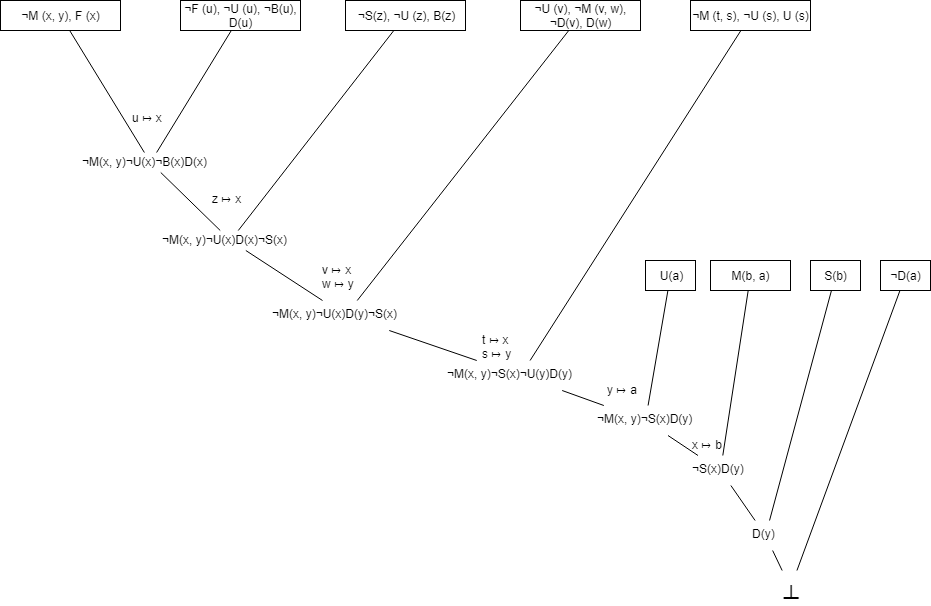
\includegraphics[width=\textwidth]{4}

\subsection*{Challenge 5 Answer Part A}
\begin{enumerate}
\setlength{\itemsep}{-0.5ex}
\item
$\forall x \forall y (N(x, y) \impl N(y, x))$ \\
\item
$\forall x \forall y (\exists u (M(u, x) \land \neg M(u, y)) \impl N(x, y))$ \\
\item
$\forall x (\exists u (\neg M(u, x)) \impl F(x))$ \\
\item
$\forall x \forall y \forall u ((D(x, y) \land M(u, x)) \impl \neg M(u, y))$
\end{enumerate}

\subsection*{Challenge 5 Answer Part B}
\begin{enumerate}
\setlength{\itemsep}{-0.5ex}
\item
$\forall x \forall y (N(x, y) \impl N(y, x))$ \\
$\forall x \forall y (\neg N(x, y) \lor N(y, x))$ \\
$\{\neg N(x, y), N(y, x)\}$ \\
\item
$\forall x \forall y (\exists u (M(u, x) \land \neg M(u, y)) \impl N(x, y))$ \\
$\forall x \forall y (\forall u (\neg M(u, x) \lor M(u, y)) \lor N(x, y))$ \\
$\{\neg M(u, x), M(u, y), N(x, y)\}$ \\
\item
$\forall x (\neg \exists u (M(u, x)) \impl E(x))$ \\
$\forall x (\neg\neg\exists u (M(u, x)) \lor E(x))$ \\
$\forall x (\exists u (M(u, x)) \lor E(x))$ \\
$\forall x ((M(f(x), x)) \lor E(x))$ \tab (skolemize)\\
$\{M(f(x), x), E(x)\}$ \\
\item
$\forall x \forall y \forall u ((D(x, y) \land M(u, x)) \impl \neg M(u, y))$ \\
$\forall x \forall y \forall u (\neg(D(x, y) \land M(u, x)) \lor \neg M(u, y))$ \\
$\forall x \forall y \forall u ((\neg D(x, y) \lor \neg M(u, x)) \lor \neg M(u, y))$ \\
$\{\neg D(x, y), \neg M(u, x), \neg M(u, y)\}$\\
\end{enumerate}

\subsection*{Challenge 5 Answer Part C}
Our fifth statement can be described by the following:\\
$\forall x \forall y (D(x, y) \impl (N(x, y) \lor (E(x) \land E(y))))$\\\\
To show this statement is a logical consequence of the statements (a1-a4), we can negate it and resolve for unsatisfiability:\\
$\neg\forall x \forall y (D(x, y) \impl (N(x, y) \lor (E(x) \land E(y))))$\\\\
$\neg\forall x \forall y (\neg D(x, y) \lor (N(x, y) \lor (E(x) \land E(y))))$\\\\
$\exists x \exists y \neg(\neg D(x, y) \lor (N(x, y) \lor (E(x) \land E(y))))$\\\\
$\exists x \exists y (\neg\neg D(x, y) \land \neg(N(x, y) \lor (E(x) \land E(y))))$\\\\
$\exists x \exists y (D(x, y) \land (\neg N(x, y) \land \neg(E(x) \land E(y))))$\\\\
$\exists x \exists y (D(x, y) \land (\neg N(x, y) \land (\neg E(x) \lor \neg E(y))))$\\\\
After Skolemization:\\
$(D(a, b) \land (\neg N(a, b) \land (\neg E(a) \lor \neg E(b))))$\\\\
$\{\{D(a, b)\}, \{\neg N(a, b)\} \{\neg E(a),\neg E(b)\}\}$\\\\
\pagebreak
\subsection*{Challenge 5 Answer Part D}
Finally, unification:\\\\
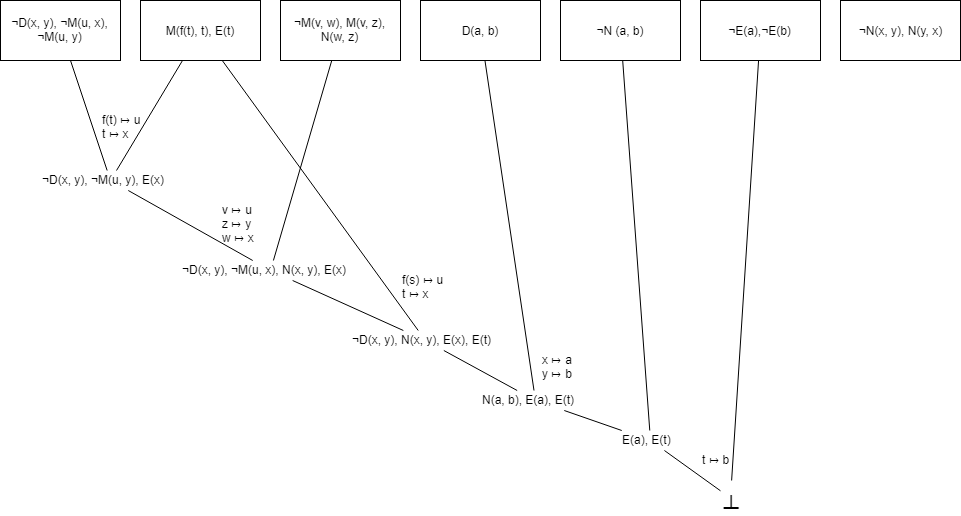
\includegraphics[width=\textwidth]{5}

\end{document}